\documentclass[11pt]{article}

    \usepackage[breakable]{tcolorbox}
    \usepackage{parskip} % Stop auto-indenting (to mimic markdown behaviour)
    
    \usepackage{iftex}
    \ifPDFTeX
    	\usepackage[T1]{fontenc}
    	\usepackage{mathpazo}
    \else
    	\usepackage{fontspec}
    \fi

    % Basic figure setup, for now with no caption control since it's done
    % automatically by Pandoc (which extracts ![](path) syntax from Markdown).
    \usepackage{graphicx}
    % Maintain compatibility with old templates. Remove in nbconvert 6.0
    \let\Oldincludegraphics\includegraphics
    % Ensure that by default, figures have no caption (until we provide a
    % proper Figure object with a Caption API and a way to capture that
    % in the conversion process - todo).
    \usepackage{caption}
    \DeclareCaptionFormat{nocaption}{}
    \captionsetup{format=nocaption,aboveskip=0pt,belowskip=0pt}

    \usepackage{float}
    \floatplacement{figure}{H} % forces figures to be placed at the correct location
    \usepackage{xcolor} % Allow colors to be defined
    \usepackage{enumerate} % Needed for markdown enumerations to work
    \usepackage{geometry} % Used to adjust the document margins
    \usepackage{amsmath} % Equations
    \usepackage{amssymb} % Equations
    \usepackage{physics}
    \usepackage{textcomp} % defines textquotesingle
    % Hack from http://tex.stackexchange.com/a/47451/13684:
    \AtBeginDocument{%
        \def\PYZsq{\textquotesingle}% Upright quotes in Pygmentized code
    }
    \usepackage{upquote} % Upright quotes for verbatim code
    \usepackage{eurosym} % defines \euro
    \usepackage[mathletters]{ucs} % Extended unicode (utf-8) support
    \usepackage{fancyvrb} % verbatim replacement that allows latex
    \usepackage{grffile} % extends the file name processing of package graphics 
                         % to support a larger range
    \makeatletter % fix for old versions of grffile with XeLaTeX
    \@ifpackagelater{grffile}{2019/11/01}
    {
      % Do nothing on new versions
    }
    {
      \def\Gread@@xetex#1{%
        \IfFileExists{"\Gin@base".bb}%
        {\Gread@eps{\Gin@base.bb}}%
        {\Gread@@xetex@aux#1}%
      }
    }
    \makeatother
    \usepackage[Export]{adjustbox} % Used to constrain images to a maximum size
    \adjustboxset{max size={0.9\linewidth}{0.9\paperheight}}

    % The hyperref package gives us a pdf with properly built
    % internal navigation ('pdf bookmarks' for the table of contents,
    % internal cross-reference links, web links for URLs, etc.)
    \usepackage{hyperref}
    % The default LaTeX title has an obnoxious amount of whitespace. By default,
    % titling removes some of it. It also provides customization options.
    \usepackage{titling}
    \usepackage{longtable} % longtable support required by pandoc >1.10
    \usepackage{booktabs}  % table support for pandoc > 1.12.2
    \usepackage[inline]{enumitem} % IRkernel/repr support (it uses the enumerate* environment)
    \usepackage[normalem]{ulem} % ulem is needed to support strikethroughs (\sout)
                                % normalem makes italics be italics, not underlines
    \usepackage{mathrsfs}
    \usepackage[version=4,arrows=pgf-filled,
textfontname=sffamily,
mathfontname=mathsf]{mhchem}
    \usepackage{mathabx}
    

    
    % Colors for the hyperref package
    \definecolor{urlcolor}{rgb}{0,.145,.698}
    \definecolor{linkcolor}{rgb}{.71,0.21,0.01}
    \definecolor{citecolor}{rgb}{.12,.54,.11}

    % ANSI colors
    \definecolor{ansi-black}{HTML}{3E424D}
    \definecolor{ansi-black-intense}{HTML}{282C36}
    \definecolor{ansi-red}{HTML}{E75C58}
    \definecolor{ansi-red-intense}{HTML}{B22B31}
    \definecolor{ansi-green}{HTML}{00A250}
    \definecolor{ansi-green-intense}{HTML}{007427}
    \definecolor{ansi-yellow}{HTML}{DDB62B}
    \definecolor{ansi-yellow-intense}{HTML}{B27D12}
    \definecolor{ansi-blue}{HTML}{208FFB}
    \definecolor{ansi-blue-intense}{HTML}{0065CA}
    \definecolor{ansi-magenta}{HTML}{D160C4}
    \definecolor{ansi-magenta-intense}{HTML}{A03196}
    \definecolor{ansi-cyan}{HTML}{60C6C8}
    \definecolor{ansi-cyan-intense}{HTML}{258F8F}
    \definecolor{ansi-white}{HTML}{C5C1B4}
    \definecolor{ansi-white-intense}{HTML}{A1A6B2}
    \definecolor{ansi-default-inverse-fg}{HTML}{FFFFFF}
    \definecolor{ansi-default-inverse-bg}{HTML}{000000}

    % common color for the border for error outputs.
    \definecolor{outerrorbackground}{HTML}{FFDFDF}

    % commands and environments needed by pandoc snippets
    % extracted from the output of `pandoc -s`
    \providecommand{\tightlist}{%
      \setlength{\itemsep}{0pt}\setlength{\parskip}{0pt}}
    \DefineVerbatimEnvironment{Highlighting}{Verbatim}{commandchars=\\\{\}}
    % Add ',fontsize=\small' for more characters per line
    \newenvironment{Shaded}{}{}
    \newcommand{\KeywordTok}[1]{\textcolor[rgb]{0.00,0.44,0.13}{\textbf{{#1}}}}
    \newcommand{\DataTypeTok}[1]{\textcolor[rgb]{0.56,0.13,0.00}{{#1}}}
    \newcommand{\DecValTok}[1]{\textcolor[rgb]{0.25,0.63,0.44}{{#1}}}
    \newcommand{\BaseNTok}[1]{\textcolor[rgb]{0.25,0.63,0.44}{{#1}}}
    \newcommand{\FloatTok}[1]{\textcolor[rgb]{0.25,0.63,0.44}{{#1}}}
    \newcommand{\CharTok}[1]{\textcolor[rgb]{0.25,0.44,0.63}{{#1}}}
    \newcommand{\StringTok}[1]{\textcolor[rgb]{0.25,0.44,0.63}{{#1}}}
    \newcommand{\CommentTok}[1]{\textcolor[rgb]{0.38,0.63,0.69}{\textit{{#1}}}}
    \newcommand{\OtherTok}[1]{\textcolor[rgb]{0.00,0.44,0.13}{{#1}}}
    \newcommand{\AlertTok}[1]{\textcolor[rgb]{1.00,0.00,0.00}{\textbf{{#1}}}}
    \newcommand{\FunctionTok}[1]{\textcolor[rgb]{0.02,0.16,0.49}{{#1}}}
    \newcommand{\RegionMarkerTok}[1]{{#1}}
    \newcommand{\ErrorTok}[1]{\textcolor[rgb]{1.00,0.00,0.00}{\textbf{{#1}}}}
    \newcommand{\NormalTok}[1]{{#1}}
    
    % Additional commands for more recent versions of Pandoc
    \newcommand{\ConstantTok}[1]{\textcolor[rgb]{0.53,0.00,0.00}{{#1}}}
    \newcommand{\SpecialCharTok}[1]{\textcolor[rgb]{0.25,0.44,0.63}{{#1}}}
    \newcommand{\VerbatimStringTok}[1]{\textcolor[rgb]{0.25,0.44,0.63}{{#1}}}
    \newcommand{\SpecialStringTok}[1]{\textcolor[rgb]{0.73,0.40,0.53}{{#1}}}
    \newcommand{\ImportTok}[1]{{#1}}
    \newcommand{\DocumentationTok}[1]{\textcolor[rgb]{0.73,0.13,0.13}{\textit{{#1}}}}
    \newcommand{\AnnotationTok}[1]{\textcolor[rgb]{0.38,0.63,0.69}{\textbf{\textit{{#1}}}}}
    \newcommand{\CommentVarTok}[1]{\textcolor[rgb]{0.38,0.63,0.69}{\textbf{\textit{{#1}}}}}
    \newcommand{\VariableTok}[1]{\textcolor[rgb]{0.10,0.09,0.49}{{#1}}}
    \newcommand{\ControlFlowTok}[1]{\textcolor[rgb]{0.00,0.44,0.13}{\textbf{{#1}}}}
    \newcommand{\OperatorTok}[1]{\textcolor[rgb]{0.40,0.40,0.40}{{#1}}}
    \newcommand{\BuiltInTok}[1]{{#1}}
    \newcommand{\ExtensionTok}[1]{{#1}}
    \newcommand{\PreprocessorTok}[1]{\textcolor[rgb]{0.74,0.48,0.00}{{#1}}}
    \newcommand{\AttributeTok}[1]{\textcolor[rgb]{0.49,0.56,0.16}{{#1}}}
    \newcommand{\InformationTok}[1]{\textcolor[rgb]{0.38,0.63,0.69}{\textbf{\textit{{#1}}}}}
    \newcommand{\WarningTok}[1]{\textcolor[rgb]{0.38,0.63,0.69}{\textbf{\textit{{#1}}}}}
    
    
    % Define a nice break command that doesn't care if a line doesn't already
    % exist.
    \def\br{\hspace*{\fill} \\* }
    % Math Jax compatibility definitions
    \def\gt{>}
    \def\lt{<}
    \let\Oldtex\TeX
    \let\Oldlatex\LaTeX
    \renewcommand{\TeX}{\textrm{\Oldtex}}
    \renewcommand{\LaTeX}{\textrm{\Oldlatex}}
    % Document parameters
    % Document title
    \title{PC3233 Assignment 6}
    
    
    
    
    
% Pygments definitions
\makeatletter
\def\PY@reset{\let\PY@it=\relax \let\PY@bf=\relax%
    \let\PY@ul=\relax \let\PY@tc=\relax%
    \let\PY@bc=\relax \let\PY@ff=\relax}
\def\PY@tok#1{\csname PY@tok@#1\endcsname}
\def\PY@toks#1+{\ifx\relax#1\empty\else%
    \PY@tok{#1}\expandafter\PY@toks\fi}
\def\PY@do#1{\PY@bc{\PY@tc{\PY@ul{%
    \PY@it{\PY@bf{\PY@ff{#1}}}}}}}
\def\PY#1#2{\PY@reset\PY@toks#1+\relax+\PY@do{#2}}

\@namedef{PY@tok@w}{\def\PY@tc##1{\textcolor[rgb]{0.73,0.73,0.73}{##1}}}
\@namedef{PY@tok@c}{\let\PY@it=\textit\def\PY@tc##1{\textcolor[rgb]{0.24,0.48,0.48}{##1}}}
\@namedef{PY@tok@cp}{\def\PY@tc##1{\textcolor[rgb]{0.61,0.40,0.00}{##1}}}
\@namedef{PY@tok@k}{\let\PY@bf=\textbf\def\PY@tc##1{\textcolor[rgb]{0.00,0.50,0.00}{##1}}}
\@namedef{PY@tok@kp}{\def\PY@tc##1{\textcolor[rgb]{0.00,0.50,0.00}{##1}}}
\@namedef{PY@tok@kt}{\def\PY@tc##1{\textcolor[rgb]{0.69,0.00,0.25}{##1}}}
\@namedef{PY@tok@o}{\def\PY@tc##1{\textcolor[rgb]{0.40,0.40,0.40}{##1}}}
\@namedef{PY@tok@ow}{\let\PY@bf=\textbf\def\PY@tc##1{\textcolor[rgb]{0.67,0.13,1.00}{##1}}}
\@namedef{PY@tok@nb}{\def\PY@tc##1{\textcolor[rgb]{0.00,0.50,0.00}{##1}}}
\@namedef{PY@tok@nf}{\def\PY@tc##1{\textcolor[rgb]{0.00,0.00,1.00}{##1}}}
\@namedef{PY@tok@nc}{\let\PY@bf=\textbf\def\PY@tc##1{\textcolor[rgb]{0.00,0.00,1.00}{##1}}}
\@namedef{PY@tok@nn}{\let\PY@bf=\textbf\def\PY@tc##1{\textcolor[rgb]{0.00,0.00,1.00}{##1}}}
\@namedef{PY@tok@ne}{\let\PY@bf=\textbf\def\PY@tc##1{\textcolor[rgb]{0.80,0.25,0.22}{##1}}}
\@namedef{PY@tok@nv}{\def\PY@tc##1{\textcolor[rgb]{0.10,0.09,0.49}{##1}}}
\@namedef{PY@tok@no}{\def\PY@tc##1{\textcolor[rgb]{0.53,0.00,0.00}{##1}}}
\@namedef{PY@tok@nl}{\def\PY@tc##1{\textcolor[rgb]{0.46,0.46,0.00}{##1}}}
\@namedef{PY@tok@ni}{\let\PY@bf=\textbf\def\PY@tc##1{\textcolor[rgb]{0.44,0.44,0.44}{##1}}}
\@namedef{PY@tok@na}{\def\PY@tc##1{\textcolor[rgb]{0.41,0.47,0.13}{##1}}}
\@namedef{PY@tok@nt}{\let\PY@bf=\textbf\def\PY@tc##1{\textcolor[rgb]{0.00,0.50,0.00}{##1}}}
\@namedef{PY@tok@nd}{\def\PY@tc##1{\textcolor[rgb]{0.67,0.13,1.00}{##1}}}
\@namedef{PY@tok@s}{\def\PY@tc##1{\textcolor[rgb]{0.73,0.13,0.13}{##1}}}
\@namedef{PY@tok@sd}{\let\PY@it=\textit\def\PY@tc##1{\textcolor[rgb]{0.73,0.13,0.13}{##1}}}
\@namedef{PY@tok@si}{\let\PY@bf=\textbf\def\PY@tc##1{\textcolor[rgb]{0.64,0.35,0.47}{##1}}}
\@namedef{PY@tok@se}{\let\PY@bf=\textbf\def\PY@tc##1{\textcolor[rgb]{0.67,0.36,0.12}{##1}}}
\@namedef{PY@tok@sr}{\def\PY@tc##1{\textcolor[rgb]{0.64,0.35,0.47}{##1}}}
\@namedef{PY@tok@ss}{\def\PY@tc##1{\textcolor[rgb]{0.10,0.09,0.49}{##1}}}
\@namedef{PY@tok@sx}{\def\PY@tc##1{\textcolor[rgb]{0.00,0.50,0.00}{##1}}}
\@namedef{PY@tok@m}{\def\PY@tc##1{\textcolor[rgb]{0.40,0.40,0.40}{##1}}}
\@namedef{PY@tok@gh}{\let\PY@bf=\textbf\def\PY@tc##1{\textcolor[rgb]{0.00,0.00,0.50}{##1}}}
\@namedef{PY@tok@gu}{\let\PY@bf=\textbf\def\PY@tc##1{\textcolor[rgb]{0.50,0.00,0.50}{##1}}}
\@namedef{PY@tok@gd}{\def\PY@tc##1{\textcolor[rgb]{0.63,0.00,0.00}{##1}}}
\@namedef{PY@tok@gi}{\def\PY@tc##1{\textcolor[rgb]{0.00,0.52,0.00}{##1}}}
\@namedef{PY@tok@gr}{\def\PY@tc##1{\textcolor[rgb]{0.89,0.00,0.00}{##1}}}
\@namedef{PY@tok@ge}{\let\PY@it=\textit}
\@namedef{PY@tok@gs}{\let\PY@bf=\textbf}
\@namedef{PY@tok@gp}{\let\PY@bf=\textbf\def\PY@tc##1{\textcolor[rgb]{0.00,0.00,0.50}{##1}}}
\@namedef{PY@tok@go}{\def\PY@tc##1{\textcolor[rgb]{0.44,0.44,0.44}{##1}}}
\@namedef{PY@tok@gt}{\def\PY@tc##1{\textcolor[rgb]{0.00,0.27,0.87}{##1}}}
\@namedef{PY@tok@err}{\def\PY@bc##1{{\setlength{\fboxsep}{\string -\fboxrule}\fcolorbox[rgb]{1.00,0.00,0.00}{1,1,1}{\strut ##1}}}}
\@namedef{PY@tok@kc}{\let\PY@bf=\textbf\def\PY@tc##1{\textcolor[rgb]{0.00,0.50,0.00}{##1}}}
\@namedef{PY@tok@kd}{\let\PY@bf=\textbf\def\PY@tc##1{\textcolor[rgb]{0.00,0.50,0.00}{##1}}}
\@namedef{PY@tok@kn}{\let\PY@bf=\textbf\def\PY@tc##1{\textcolor[rgb]{0.00,0.50,0.00}{##1}}}
\@namedef{PY@tok@kr}{\let\PY@bf=\textbf\def\PY@tc##1{\textcolor[rgb]{0.00,0.50,0.00}{##1}}}
\@namedef{PY@tok@bp}{\def\PY@tc##1{\textcolor[rgb]{0.00,0.50,0.00}{##1}}}
\@namedef{PY@tok@fm}{\def\PY@tc##1{\textcolor[rgb]{0.00,0.00,1.00}{##1}}}
\@namedef{PY@tok@vc}{\def\PY@tc##1{\textcolor[rgb]{0.10,0.09,0.49}{##1}}}
\@namedef{PY@tok@vg}{\def\PY@tc##1{\textcolor[rgb]{0.10,0.09,0.49}{##1}}}
\@namedef{PY@tok@vi}{\def\PY@tc##1{\textcolor[rgb]{0.10,0.09,0.49}{##1}}}
\@namedef{PY@tok@vm}{\def\PY@tc##1{\textcolor[rgb]{0.10,0.09,0.49}{##1}}}
\@namedef{PY@tok@sa}{\def\PY@tc##1{\textcolor[rgb]{0.73,0.13,0.13}{##1}}}
\@namedef{PY@tok@sb}{\def\PY@tc##1{\textcolor[rgb]{0.73,0.13,0.13}{##1}}}
\@namedef{PY@tok@sc}{\def\PY@tc##1{\textcolor[rgb]{0.73,0.13,0.13}{##1}}}
\@namedef{PY@tok@dl}{\def\PY@tc##1{\textcolor[rgb]{0.73,0.13,0.13}{##1}}}
\@namedef{PY@tok@s2}{\def\PY@tc##1{\textcolor[rgb]{0.73,0.13,0.13}{##1}}}
\@namedef{PY@tok@sh}{\def\PY@tc##1{\textcolor[rgb]{0.73,0.13,0.13}{##1}}}
\@namedef{PY@tok@s1}{\def\PY@tc##1{\textcolor[rgb]{0.73,0.13,0.13}{##1}}}
\@namedef{PY@tok@mb}{\def\PY@tc##1{\textcolor[rgb]{0.40,0.40,0.40}{##1}}}
\@namedef{PY@tok@mf}{\def\PY@tc##1{\textcolor[rgb]{0.40,0.40,0.40}{##1}}}
\@namedef{PY@tok@mh}{\def\PY@tc##1{\textcolor[rgb]{0.40,0.40,0.40}{##1}}}
\@namedef{PY@tok@mi}{\def\PY@tc##1{\textcolor[rgb]{0.40,0.40,0.40}{##1}}}
\@namedef{PY@tok@il}{\def\PY@tc##1{\textcolor[rgb]{0.40,0.40,0.40}{##1}}}
\@namedef{PY@tok@mo}{\def\PY@tc##1{\textcolor[rgb]{0.40,0.40,0.40}{##1}}}
\@namedef{PY@tok@ch}{\let\PY@it=\textit\def\PY@tc##1{\textcolor[rgb]{0.24,0.48,0.48}{##1}}}
\@namedef{PY@tok@cm}{\let\PY@it=\textit\def\PY@tc##1{\textcolor[rgb]{0.24,0.48,0.48}{##1}}}
\@namedef{PY@tok@cpf}{\let\PY@it=\textit\def\PY@tc##1{\textcolor[rgb]{0.24,0.48,0.48}{##1}}}
\@namedef{PY@tok@c1}{\let\PY@it=\textit\def\PY@tc##1{\textcolor[rgb]{0.24,0.48,0.48}{##1}}}
\@namedef{PY@tok@cs}{\let\PY@it=\textit\def\PY@tc##1{\textcolor[rgb]{0.24,0.48,0.48}{##1}}}

\def\PYZbs{\char`\\}
\def\PYZus{\char`\_}
\def\PYZob{\char`\{}
\def\PYZcb{\char`\}}
\def\PYZca{\char`\^}
\def\PYZam{\char`\&}
\def\PYZlt{\char`\<}
\def\PYZgt{\char`\>}
\def\PYZsh{\char`\#}
\def\PYZpc{\char`\%}
\def\PYZdl{\char`\$}
\def\PYZhy{\char`\-}
\def\PYZsq{\char`\'}
\def\PYZdq{\char`\"}
\def\PYZti{\char`\~}
% for compatibility with earlier versions
\def\PYZat{@}
\def\PYZlb{[}
\def\PYZrb{]}
\makeatother


    % For linebreaks inside Verbatim environment from package fancyvrb. 
    \makeatletter
        \newbox\Wrappedcontinuationbox 
        \newbox\Wrappedvisiblespacebox 
        \newcommand*\Wrappedvisiblespace {\textcolor{red}{\textvisiblespace}} 
        \newcommand*\Wrappedcontinuationsymbol {\textcolor{red}{\llap{\tiny$\m@th\hookrightarrow$}}} 
        \newcommand*\Wrappedcontinuationindent {3ex } 
        \newcommand*\Wrappedafterbreak {\kern\Wrappedcontinuationindent\copy\Wrappedcontinuationbox} 
        % Take advantage of the already applied Pygments mark-up to insert 
        % potential linebreaks for TeX processing. 
        %        {, <, #, %, $, ' and ": go to next line. 
        %        _, }, ^, &, >, - and ~: stay at end of broken line. 
        % Use of \textquotesingle for straight quote. 
        \newcommand*\Wrappedbreaksatspecials {% 
            \def\PYGZus{\discretionary{\char`\_}{\Wrappedafterbreak}{\char`\_}}% 
            \def\PYGZob{\discretionary{}{\Wrappedafterbreak\char`\{}{\char`\{}}% 
            \def\PYGZcb{\discretionary{\char`\}}{\Wrappedafterbreak}{\char`\}}}% 
            \def\PYGZca{\discretionary{\char`\^}{\Wrappedafterbreak}{\char`\^}}% 
            \def\PYGZam{\discretionary{\char`\&}{\Wrappedafterbreak}{\char`\&}}% 
            \def\PYGZlt{\discretionary{}{\Wrappedafterbreak\char`\<}{\char`\<}}% 
            \def\PYGZgt{\discretionary{\char`\>}{\Wrappedafterbreak}{\char`\>}}% 
            \def\PYGZsh{\discretionary{}{\Wrappedafterbreak\char`\#}{\char`\#}}% 
            \def\PYGZpc{\discretionary{}{\Wrappedafterbreak\char`\%}{\char`\%}}% 
            \def\PYGZdl{\discretionary{}{\Wrappedafterbreak\char`\$}{\char`\$}}% 
            \def\PYGZhy{\discretionary{\char`\-}{\Wrappedafterbreak}{\char`\-}}% 
            \def\PYGZsq{\discretionary{}{\Wrappedafterbreak\textquotesingle}{\textquotesingle}}% 
            \def\PYGZdq{\discretionary{}{\Wrappedafterbreak\char`\"}{\char`\"}}% 
            \def\PYGZti{\discretionary{\char`\~}{\Wrappedafterbreak}{\char`\~}}% 
        } 
        % Some characters . , ; ? ! / are not pygmentized. 
        % This macro makes them "active" and they will insert potential linebreaks 
        \newcommand*\Wrappedbreaksatpunct {% 
            \lccode`\~`\.\lowercase{\def~}{\discretionary{\hbox{\char`\.}}{\Wrappedafterbreak}{\hbox{\char`\.}}}% 
            \lccode`\~`\,\lowercase{\def~}{\discretionary{\hbox{\char`\,}}{\Wrappedafterbreak}{\hbox{\char`\,}}}% 
            \lccode`\~`\;\lowercase{\def~}{\discretionary{\hbox{\char`\;}}{\Wrappedafterbreak}{\hbox{\char`\;}}}% 
            \lccode`\~`\:\lowercase{\def~}{\discretionary{\hbox{\char`\:}}{\Wrappedafterbreak}{\hbox{\char`\:}}}% 
            \lccode`\~`\?\lowercase{\def~}{\discretionary{\hbox{\char`\?}}{\Wrappedafterbreak}{\hbox{\char`\?}}}% 
            \lccode`\~`\!\lowercase{\def~}{\discretionary{\hbox{\char`\!}}{\Wrappedafterbreak}{\hbox{\char`\!}}}% 
            \lccode`\~`\/\lowercase{\def~}{\discretionary{\hbox{\char`\/}}{\Wrappedafterbreak}{\hbox{\char`\/}}}% 
            \catcode`\.\active
            \catcode`\,\active 
            \catcode`\;\active
            \catcode`\:\active
            \catcode`\?\active
            \catcode`\!\active
            \catcode`\/\active 
            \lccode`\~`\~ 	
        }
    \makeatother

    \let\OriginalVerbatim=\Verbatim
    \makeatletter
    \renewcommand{\Verbatim}[1][1]{%
        %\parskip\z@skip
        \sbox\Wrappedcontinuationbox {\Wrappedcontinuationsymbol}%
        \sbox\Wrappedvisiblespacebox {\FV@SetupFont\Wrappedvisiblespace}%
        \def\FancyVerbFormatLine ##1{\hsize\linewidth
            \vtop{\raggedright\hyphenpenalty\z@\exhyphenpenalty\z@
                \doublehyphendemerits\z@\finalhyphendemerits\z@
                \strut ##1\strut}%
        }%
        % If the linebreak is at a space, the latter will be displayed as visible
        % space at end of first line, and a continuation symbol starts next line.
        % Stretch/shrink are however usually zero for typewriter font.
        \def\FV@Space {%
            \nobreak\hskip\z@ plus\fontdimen3\font minus\fontdimen4\font
            \discretionary{\copy\Wrappedvisiblespacebox}{\Wrappedafterbreak}
            {\kern\fontdimen2\font}%
        }%
        
        % Allow breaks at special characters using \PYG... macros.
        \Wrappedbreaksatspecials
        % Breaks at punctuation characters . , ; ? ! and / need catcode=\active 	
        \OriginalVerbatim[#1,codes*=\Wrappedbreaksatpunct]%
    }
    \makeatother

    % Exact colors from NB
    \definecolor{incolor}{HTML}{303F9F}
    \definecolor{outcolor}{HTML}{D84315}
    \definecolor{cellborder}{HTML}{CFCFCF}
    \definecolor{cellbackground}{HTML}{F7F7F7}
    
    % prompt
    \makeatletter
    \newcommand{\boxspacing}{\kern\kvtcb@left@rule\kern\kvtcb@boxsep}
    \makeatother
    \newcommand{\prompt}[4]{
        {\ttfamily\llap{{\color{#2}[#3]:\hspace{3pt}#4}}\vspace{-\baselineskip}}
    }
    

    
    % Prevent overflowing lines due to hard-to-break entities
    \sloppy 
    % Setup hyperref package
    \hypersetup{
      breaklinks=true,  % so long urls are correctly broken across lines
      colorlinks=true,
      urlcolor=urlcolor,
      linkcolor=linkcolor,
      citecolor=citecolor,
      }
    % Slightly bigger margins than the latex defaults
    
    \geometry{verbose,tmargin=1in,bmargin=1in,lmargin=1in,rmargin=1in}
    
    

\begin{document}
    
    \maketitle
    
    \section{Atom in magnetic fields}

    Consider an atom in an electronically excited fine-structure state \texorpdfstring{${}^{4}D_{1/2}$}{4D1/2}. We
    know that the quantum number $s = \frac{3}{2}, l = 2, j = \frac{1}{2}$.

    Suppose the coupling effect of nuclear spin is negligible, the energy splitting in magnetic field is given by:

    \begin{equation}
      \Delta E = \Delta m_j g_j \mu_B B
    \end{equation}

    The Lande g-factor, $g_j$ is given by:

    \begin{equation}
      g_j = 1 + \frac{j(j+1) + s(s+1) - l(l+1)}{2j(j+1)}
    \end{equation}

    Substitute the quantum numbers into the equation gives:

    \begin{equation}
      g_j = 1 + \frac{\frac{1}{2}(\frac{1}{2}+1) + \frac{3}{2}(\frac{3}{2}+1) - 2(2+1)}{2\frac{1}{2}(\frac{1}{2}+1)} = 0
    \end{equation}

    Lande g-factor is zero, implies that the energy splitting in magnetic field is zero.

    \section{$\ce{^{4}He}$ atom}

    \subsection{Separable Wavefunction and Energy}

    From lecture, we know that the general Schrodinger equation for Helium atom is given by:

    \begin{equation}
      - \frac{\hbar^{2}}{2m_e}\Delta_1 \psi(\vb{r}_{1}, \vb{r}_{2}) 
      - \frac{\hbar^{2}}{2m_e}\Delta_2 \psi(\vb{r}_{1}, \vb{r}_{2})
      + E_{\text{pot}}\psi(\vb{r}_{1}, \vb{r}_{2}) = E\psi(\vb{r}_{1}, \vb{r}_{2})
    \end{equation}

    The $E_{\text{pot}}$ term is the potential energy is given by:

    \begin{equation}
      E_{\text{pot}} = - \frac{e^{2}}{4\pi\epsilon_0} \left( \frac{1}{r_1} + \frac{1}{r_2} - \frac{1}{r_{12}}\right)
    \end{equation}

    Assuming the mutual replusion between the electrons is negligible, we can drop the $1/r_{12}$ term. 
    Therefore, the potential energy term simplifies to:

    \begin{equation}
      E_{\text{pot}} = - \frac{e^{2}}{4\pi\epsilon_0} \left( \frac{1}{r_1} + \frac{1}{r_2}\right)
    \end{equation}

    Substitute the potential energy term into the Schrodinger equation gives:

    \begin{equation}
      - \frac{\hbar^{2}}{2m_e}\Delta_1 \psi(\vb{r}_{1}) 
      - \frac{\hbar^{2}}{2m_e}\Delta_2 \psi(\vb{r}_{2})
      - \frac{e^{2}}{4\pi\epsilon_0} \left( \frac{1}{r_1} + \frac{1}{r_2}\right)\psi(\vb{r}_{1}, \vb{r}_{2}) 
      = E\psi(\vb{r}_{1}, \vb{r}_{2})
    \end{equation}

    Assuming the wavefunction is separable, $\psi(\vb{r}_{1}, \vb{r}_{2}) = \psi(\vb{r}_{1})\psi(\vb{r}_{2})$, 
    we can rewrite the Schrodinger equation as:

    \begin{equation}
      - \frac{\hbar^{2}}{2m_e}\Delta_1 \psi(\vb{r}_{1})\psi(\vb{r}_{2})  
      - \frac{\hbar^{2}}{2m_e}\Delta_2 \psi(\vb{r}_{1})\psi(\vb{r}_{2}) 
      - \frac{e^{2}}{4\pi\epsilon_0} \left( \frac{1}{r_1} + \frac{1}{r_2}\right)\psi(\vb{r}_{1})\psi(\vb{r}_{2}) 
      = E\psi(\vb{r}_{1})\psi(\vb{r}_{2}) 
    \end{equation}

    Dividing the equation by $\psi(\vb{r}_{1})\psi(\vb{r}_{2})$ gives:

    \begin{equation}
      - \frac{\hbar^{2}}{2m_e}\frac{\Delta_1 \psi(\vb{r}_{1})}{\psi(\vb{r}_{1})}  
      - \frac{\hbar^{2}}{2m_e}\frac{\Delta_2 \psi(\vb{r}_{2})}{\psi(\vb{r}_{2})} 
      - \frac{e^{2}}{4\pi\epsilon_0} \left( \frac{1}{r_1} + \frac{1}{r_2}\right) 
      = E
    \end{equation}

    Rearrange the equation gives:

    \begin{equation}
      - \frac{\hbar^{2}}{2m_e}\frac{\Delta_1 \psi(\vb{r}_{1})}{\psi(\vb{r}_{1})} 
      - \frac{e^{2}}{4\pi\epsilon_0} \frac{1}{r_1} 
      - \frac{\hbar^{2}}{2m_e}\frac{\Delta_2 \psi(\vb{r}_{2})}{\psi(\vb{r}_{2})}
      - \frac{e^{2}}{4\pi\epsilon_0} \frac{1}{r_2}
      = E_1
    \end{equation}

    The equation can be separated into two equations:

    \begin{equation}
      - \frac{\hbar^{2}}{2m_e}\frac{\Delta_1 \psi(\vb{r}_{1})}{\psi(\vb{r}_{1})} 
      - \frac{e^{2}}{4\pi\epsilon_0} \frac{1}{r_1} 
      = E_1
    \end{equation}

    \begin{equation}
      - \frac{\hbar^{2}}{2m_e}\frac{\Delta_2 \psi(\vb{r}_{2})}{\psi(\vb{r}_{2})}
      - \frac{e^{2}}{4\pi\epsilon_0} \frac{1}{r_2}
      = E_2
    \end{equation}

    where $E_1 + E_2 = E$.

    Hence, the energy of the Helium atom is separable into two parts, $E_1$ and $E_2$.

    \newpage

    \subsection{Potential Graph}

    Coloumb Potential is given by:

    \begin{equation}
      V(r,Z,S) = - \frac{Q_{\text{eff}}(Z, S)}{4\pi\epsilon_0} \frac{1}{r}
    \end{equation}

    where $Q_{\text{eff}}(Z, S) = (Z - S)e$, $S$ is the shielding constant.

    The potential graph for the Helium atom is shown below:

    \begin{figure}[H]
      \centering
      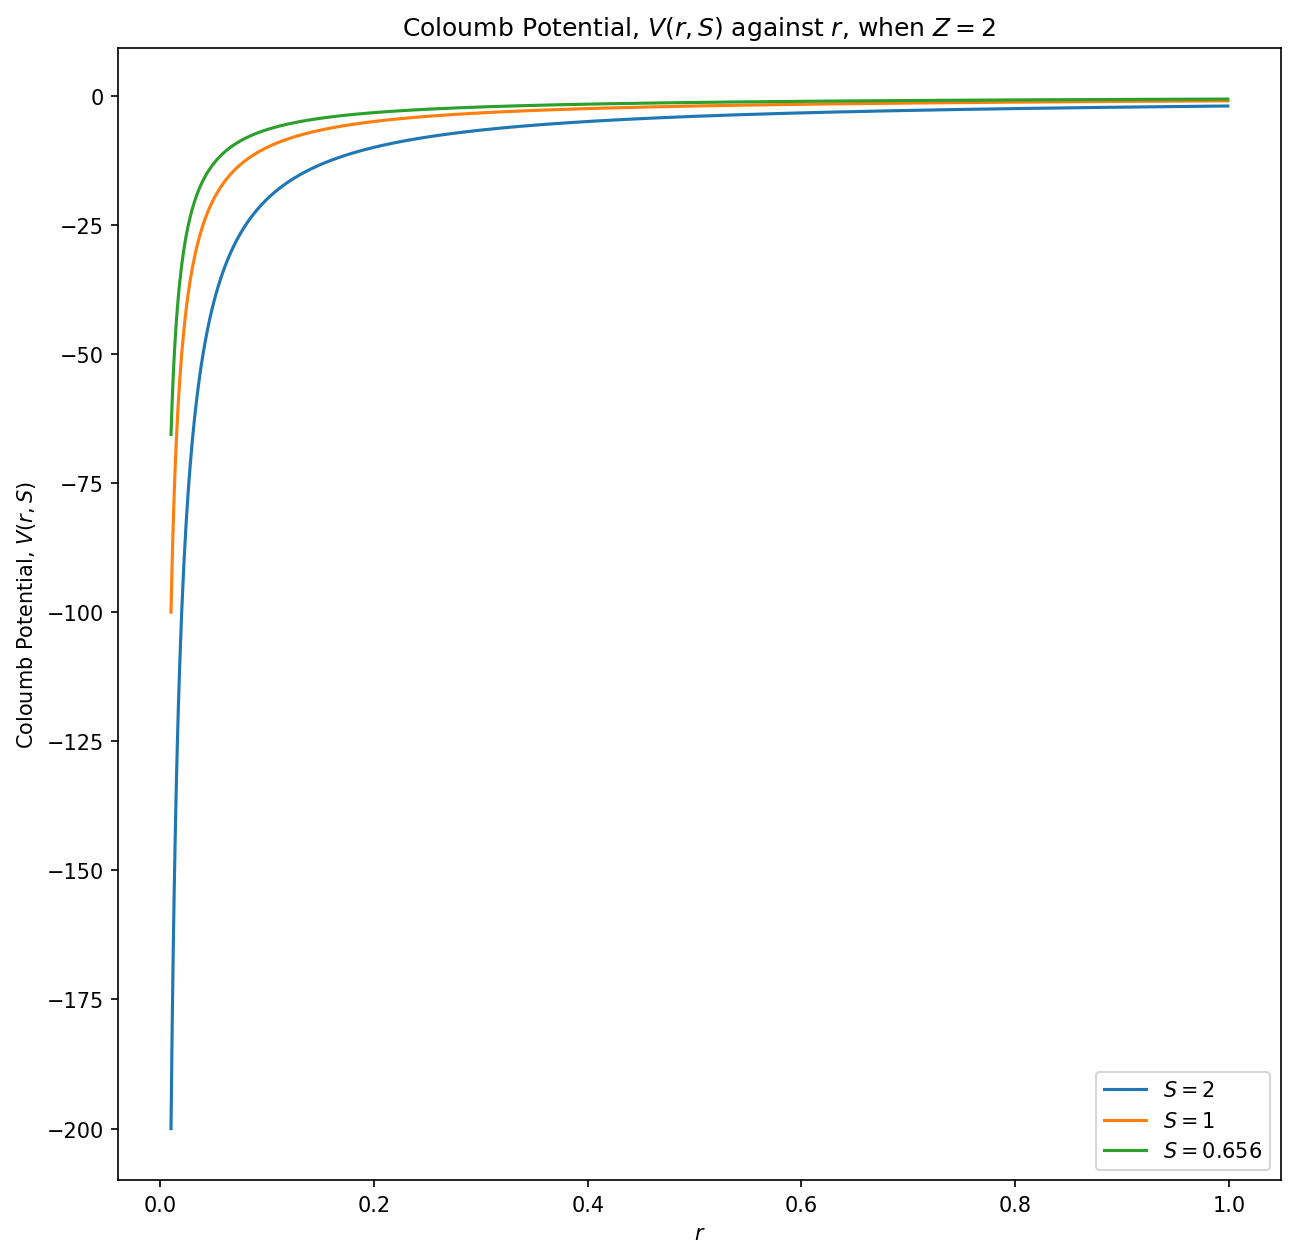
\includegraphics[width=1\textwidth]{../image/Coloumb_Potential_Assignment_6.png}
      \caption{Potential graph for Helium atom, $Z = 2$, $S = 1, 0.656, 0$}
    \end{figure}

    \section{Helium atoms}

    The energy to ionize a Helium atom is given by:

    \begin{equation}
      E_{} = E_{\text{He} \rightarrow \text{He}^{+}} + E_{\text{He}^{+} \rightarrow \text{He}^{2+}}
    \end{equation}

    We already know that the ionization energy for the first electron, $E_{\text{He} \rightarrow \text{He}^{+}}$, is $24.6$ eV. After
    the first electron is removed, the \ce{He+} ion has a single electron, which is hydrogen-like. The ionization
    energy for the hydrogen-like atom is given by:

    \begin{equation}
      E_n = - R_y^* \frac{Z^{*2}}{n^{2}}
    \end{equation}

    In this case, $Z^{*} = 2$ and $n = 1$. Therefore, the ionization energy for the \ce{He+} ion is:

    \begin{equation}
      E_{\text{He}^{+} \rightarrow \text{He}^{2+}} = - R_y^* \frac{2^{2}}{1^{2}} = - 4 \times 13.6 \text{ eV} = - 54.4 \text{ eV}
    \end{equation}

    Hence, the total ionization energy for the Helium atom is:

    \begin{equation}
      E_{} = 24.6 \text{ eV} + 54.4 \text{ eV} = 79 \text{ eV}
    \end{equation}

    \section{Two spins}

     Following the lecture note notation, we introduce spinor vectors 
     \begin{align*}
        & \chi^{m_s = +\frac{1}{2}}(\text{Hilbert Space } 1) = \chi^+(1) \\
        & \chi^{m_s = -\frac{1}{2}}(\text{Hilbert Space } 1) = \chi^-(1) \\
        & \chi^{m_s = +\frac{1}{2}}(\text{Hilbert Space } 2) = \chi^+(2) \\
        & \chi^{m_s = -\frac{1}{2}}(\text{Hilbert Space } 2) = \chi^-(2) \\
     \end{align*}

     The spin function for the two electrons is given by:
     \begin{align*}
        \chi^+(1)\chi^+(2) & = \chi^+(1)\chi^+(2) = \ket{\upuparrows} \\
        \chi^+(1)\chi^-(2) & = \chi^+(1)\chi^-(2) = \frac{1}{\sqrt{2}}(\ket{\updownarrows} + \ket{\downuparrows}) \\
        \chi^-(1)\chi^+(2) & = \chi^-(1)\chi^+(2) = \frac{1}{\sqrt{2}}(\ket{\updownarrows} - \ket{\downuparrows}) \\
        \chi^-(1)\chi^-(2) & = \chi^-(1)\chi^-(2) = \ket{\downdownarrows} \\
     \end{align*}
     We know that the total spin angular momentum operator is given by:
      \begin{equation}
          \vb{S} = \vb{S}(1) + \vb{S}(2)
      \end{equation}

      To determine the expectation value of $\vb{S}_z$:

      \begin{equation}
          \langle \vb{S}_z \rangle = \langle \vb{S}_z(1) + \vb{S}_z(2) \rangle = \langle \vb{S}_z(1) \rangle + \langle \vb{S}_z(2) \rangle = \hbar[m_s(1) + m_s(2)]
      \end{equation}

      Therefore, the expectation value of $\vb{S}_z$ for single state and all the triplet states are:

      \begin{equation}
      \begin{cases}
          \displaystyle
          \langle \vb{S}_z \rangle = \hbar \left( \frac{1}{2} + \frac{1}{2} \right) = \hbar & \text{for } \ket{\upuparrows} \\
          \displaystyle
          \langle \vb{S}_z \rangle = \hbar \left( \frac{1}{2} - \frac{1}{2} \right) = 0 &  \text{for } \frac{1}{\sqrt{2}}(\ket{\updownarrows} + \ket{\downuparrows}) \\
          \displaystyle
          \langle \vb{S}_z \rangle = \hbar \left( -\frac{1}{2} + \frac{1}{2} \right) = 0 & \text{for } \frac{1}{\sqrt{2}}(\ket{\updownarrows} - \ket{\downuparrows}) \\
          \displaystyle
          \langle \vb{S}_z \rangle = \hbar \left( -\frac{1}{2} - \frac{1}{2} \right) = -\hbar & \text{for } \ket{\downdownarrows} \\
      \end{cases}
      \end{equation}

      For $\vb{S}^2$ operator, the expectation value is given by:

      \begin{align}
          \langle \vb{S}^2 \rangle 
          &= \langle \vb{S}^2(1) + \vb{S}^2(2) + 2\vb{S}(1)\cdot\vb{S}(2) \rangle \\
          &= \langle \vb{S}^2(1) \rangle + \langle \vb{S}^2(2) \rangle + 2\langle \vb{S}(1)\cdot\vb{S}(2) \rangle
      \end{align}

      Since $\vb{S}(i) = \vb{S_x}(i) + \vb{S_y}(i) + \vb{S_z}(i)$, the dot product of $\vb{S}(1)$ and $\vb{S}(2)$ is given by:

      \begin{equation}
          \vb{S}(1)\cdot\vb{S}(2) = \vb{S_x}(1)\vb{S_x}(2) + \vb{S_y}(1)\vb{S_y}(2) + \vb{S_z}(1)\vb{S_z}(2)
      \end{equation}

      We know that $\vb{S_x} = \frac{\vb{S_+} + \vb{S_-}}{2}$, $\vb{S_y} = \frac{\vb{S_+} - \vb{S_-}}{2i}$, and $\vb{S_z} = \frac{S_+S_-}{\hbar}$. 
      Therefore, we can rewrite the expression in $(22)$ as:

      \begin{align*}
        &\langle \vb{S}^2(1) \rangle + \langle \vb{S}^2(2) \rangle + 2\langle \vb{S}(1)\cdot\vb{S}(2) \rangle \\
        &= \langle \vb{S}^2(1) \rangle + \langle \vb{S}^2(2) \rangle + 2\langle \vb{S_x}(1)\vb{S_x}(2) + \vb{S_y}(1)\vb{S_y}(2) + \vb{S_z}(1)\vb{S_z}(2) \rangle \\
        &= \langle \vb{S}^2(1) \rangle + \langle \vb{S}^2(2) \rangle + 2\langle \frac{\vb{S_+}(1) + \vb{S_-}(1)}{2} \frac{\vb{S_+}(2) + \vb{S_-}(2)}{2} + \frac{\vb{S_+}(1) - \vb{S_-}(1)}{2i} \frac{\vb{S_+}(2) - \vb{S_-}(2)}{2i} + \vb{S_z}(1)\vb{S_z}(2) \rangle \\
      \end{align*}

      Since $\vb{S_+}\ket{\uparrow} = 0$, $\vb{S_-}\ket{\downarrow} = 0$, and $\vb{S_+}\ket{\downarrow} = \vb{S_-}\ket{\uparrow} = \frac{\hbar^2}{2}$.

      We can then compute the expectation value of $\vb{S}^2$ for each state:

      \begin{equation}
        \begin{cases}
            \displaystyle
            \langle \vb{S}^2 \rangle = 2\hbar^2 & \text{for } \ket{\upuparrows} \\
            \displaystyle
            \langle \vb{S}^2 \rangle = 2\hbar^2 & \text{for } \frac{1}{\sqrt{2}}(\ket{\updownarrows} + \ket{\downuparrows}) \\
            \displaystyle
            \langle \vb{S}^2 \rangle = 0 & \text{for } \frac{1}{\sqrt{2}}(\ket{\updownarrows} - \ket{\downuparrows}) \\
            \displaystyle
            \langle \vb{S}^2 \rangle = 2\hbar^2 & \text{for } \ket{\downdownarrows} \\
        \end{cases}
      \end{equation}

\end{document}
